% \documentclass[handout]{beamer}
\documentclass{beamer}

\mode<presentation>
\usefonttheme{structurebold}
\mode<presentation>
{
  \usetheme{default}
   \setbeamercolor{structure}{fg=black!70}
  \setbeamercovered{invisible}
  \setbeamerfont{title}{size=\large}

}

\usepackage[english]{babel}
\usepackage[latin1]{inputenc}
\usepackage{textpos,alltt,listings,multirow,ulem,siunitx}
\usepackage{pdfpages}
\usepackage{multimedia}
\newcommand\hmmax{0}
\newcommand\bmmax{0}
\usepackage{bm}

% font definitions, try \usepackage{ae} instead of the following
% three lines if you don't like this look
\usepackage{mathptmx}
\usepackage[scaled=.90]{helvet}
% \usepackage{courier}
\usepackage[T1]{fontenc}
\usepackage{tikz}
\usetikzlibrary[shapes,shapes.arrows,arrows,shapes.misc,fit,positioning,trees,mindmap,backgrounds]

% \usepackage{pgfpages}
% \pgfpagesuselayout{4 on 1}[a4paper,landscape,border shrink=5mm]

\usepackage{JedMacros}
\usepackage{ctmmath-v3}

\title{Preconditioner Scaling for Finite Element Models of Turbulent Air/Water Flow in Coastal and Hydraulic Applications}
\author{{\bf Christopher E. Kees}\inst{1},\\
Aron J. Ahmadia\inst{1}, Jed Brown\inst{2}, Matthew Farthing \inst{1} Barry Smith\inst{2}}


% - Use the \inst command only if there are several affiliations.
% - Keep it simple, no one is interested in your street address.
\institute
{
  \inst{2}{Coastal and Hydraulics Laboratory, US Army Engineer
    Research and Development Center} \\
  \inst{3}{Mathematics and Computer Science Division, Argonne National Laboratory} \\
}

\date{SIAM CSE 2015-03-18}

% This is only inserted into the PDF information catalog. Can be left
% out.
\subject{Talks}


% If you have a file called "university-logo-filename.xxx", where xxx
% is a graphic format that can be processed by latex or pdflatex,
% resp., then you can add a logo as follows:

% \pgfdeclareimage[height=0.5cm]{university-logo}{university-logo-filename}
% \logo{\pgfuseimage{university-logo}}
\pgfdeclareimage[height=0.5cm]{corps_logo}{./logos/corps_logo.pdf}
\logo{\pgfuseimage{corps_logo}}



% Delete this, if you do not want the table of contents to pop up at
% the beginning of each subsection:
% \AtBeginSubsection[]
% {
% \begin{frame}<beamer>
%   \frametitle{Outline}
%   \tableofcontents[currentsection,currentsubsection]
% \end{frame}
% }

\AtBeginSection[]
{
  \begin{frame}<beamer>
    \frametitle{Outline}
    \tableofcontents[currentsection]
  \end{frame}
}

% If you wish to uncover everything in a step-wise fashion, uncomment
% the following command:

% \beamerdefaultoverlayspecification{<+->}

\begin{document}
\def\Tiny{\fontsize{4pt}{4pt}\selectfont}
\defbeamertemplate{footline}{dist}{{\Tiny DISTRIBUTION STATEMENT A: Approved for public release; distribution is unlimited.}}
\setbeamertemplate{footline}[dist]{}

\lstset{language=C}
\normalem

\begin{frame}
  \titlepage
\end{frame}

\begin{frame}{Definitions}
\begin{description}
\item [$\rho$] density
\item[$t$] time
\item[$\vec u$] fluid velocity
\item[$p$] fluid pressure
\item[$\mu$] dynamic viscosity
\item[$\vec g$] gravitational acceleration vector.
\end{description}
\end{frame}
\begin{frame}{Governing Equations}
  \begin{block}{Navier Stokes - immiscible, incompressible fluids}
    \vspace{-1em}
    \begin{align*}
      \pdt{\lrp{\rho\vec u}}
      +\rho\vec u \cdot \del\vec u + \del p -
      \deld2\mu\del^s\vec u = \rho\vec f \\
      \deld \vec u = 0
    \end{align*}
  \end{block}
  \begin{block}{Level set boundary}
    \begin{align*}
      \pdt{\phi} + \vec u \cdot \del\phi = 0 \text{ in } \Omega
    \end{align*}
  \end{block}
      \vspace{-0.8em}
  {\scriptsize (Kees, Akkerman, Farthing, Bazilevs. \emph{A
      conservative level set method suitable for variable-order
      approximations and unstructured meshes}. 2011)}
\end{frame}

\begin{frame}{Multi-physics coupling in PETSc}
  \begin{columns}
    \begin{column}{0.5\textwidth}
      \tikzstyle{cloud} = [draw, ellipse,fill=red!20, node distance=3cm, minimum height=2em]
      \tikzstyle{block} = [rectangle, draw, fill=blue!20, text width=5em, text centered, rounded corners, minimum height=2em]
      \begin{tikzpicture}
        \node [cloud] (momentum) {Momentum};
        \node [cloud, right of=momentum] (pressure) {Pressure};
        \node<2-> [block, opacity=0.5, fit=(momentum)(pressure), text opacity=0.8] (stokes) {Stokes};
        % ]
      \end{tikzpicture}
    \end{column}
    \begin{column}{0.5\textwidth}
      \begin{itemize}
      \item package each ``physics'' independently
      \item solve single-physics and coupled problems
      \item semi-implicit and fully implicit
      \item reuse residual and Jacobian evaluation unmodified
      \item direct solvers, fieldsplit inside multigrid, multigrid inside fieldsplit without recompilation
      \item use the best possible matrix format for each physics \\ (e.g. symmetric block size 3)
      \item matrix-free anywhere
      \item multiple levels of nesting
      \end{itemize}
    \end{column}
  \end{columns}
\end{frame}

\begin{frame}{Splitting for Multiphysics}
  \begin{equation*}
    \begin{bmatrix}
      A & B \\ C & D
    \end{bmatrix}
    \begin{bmatrix}
      V \\ P
    \end{bmatrix}
    =
    \begin{bmatrix}
\frac{\partial F^u}{\partial U} & \frac{\partial F^u}{\partial P}\\ \frac{\partial F^p}{\partial U} & \frac{\partial F^p}{\partial P}
    \end{bmatrix}
    \begin{bmatrix}
      V \\ P
    \end{bmatrix}
    =
    \begin{bmatrix}
      f \\ g
    \end{bmatrix}
  \end{equation*}
  \begin{itemize}\item Relaxation:
    \code{-pc\_fieldsplit\_type [additive,multiplicative,symmetric\_multiplicative]}
    \begin{equation*}
      \begin{bmatrix}
        A & \\  & D
      \end{bmatrix}^{-1} \qquad 
      \begin{bmatrix}
        A & \\ C & D
      \end{bmatrix}^{-1} \qquad
      \begin{bmatrix}
        A & \\  & \bm 1
      \end{bmatrix}^{-1}
      \left(
        \bm 1 -
        \begin{bmatrix}
          A & B \\ & \bm 1
        \end{bmatrix}
        \begin{bmatrix}
          A & \\ C & D
        \end{bmatrix}^{-1}
      \right)
    \end{equation*}
    \begin{itemize}
    \item Gauss-Seidel inspired, works when fields are loosely coupled
    \end{itemize}
  \item Factorization: \code{-pc\_fieldsplit\_type schur}
    \begin{align*}
      \begin{bmatrix}
        A & B \\ & S
      \end{bmatrix}^{-1}
      \begin{bmatrix}
        1 & \\ CA^{-1} & 1
      \end{bmatrix}^{-1}, \qquad
      S = D - C A^{-1} B
    \end{align*}
    \begin{itemize}
    \item robust (exact factorization), can often drop lower block
    \item how to precondition $S$ which is usually dense?
      \begin{itemize}
      \item interpret as differential operators, use approximate commutators
      \end{itemize}
    \end{itemize}
  \item ``Composable Linear Solvers for Multiphysics'' ISPDC 2012
  \end{itemize}
\end{frame}

\begin{frame}[shrink]{Schur Complement Preconditioners}
  \begin{equation*}
    \begin{bmatrix}
      A & B \\ C & D
    \end{bmatrix}
    \begin{bmatrix}
      x \\ y
    \end{bmatrix}
    =
    \begin{bmatrix}
      f \\ g
    \end{bmatrix}
  \end{equation*}
  \begin{block}{Full}
    \begin{align*}
      S_p = D - C A^{-1} B
    \end{align*}
  \end{block}
\begin{block}{SIMPLE-type (selfp)}
  \begin{align*}
      S_p =  D - C\ \text{diag}\left(A\right)^{-1} B
    \end{align*}
  \end{block}
  \begin{block}{Single Block (A11)}
    \begin{align*}
      S_p = D 
    \end{align*}
  \end{block}
\end{frame}


\begin{frame}{Existing Approach (Proteus ASM)}
  \begin{itemize}
  \item[] \code{-ksp\_type gmres}
  \item[] \code{-ksp\_gmres\_modifiedgramschmidt}
  \item[] \code{-ksp\_gmres\_restart 300}
  \item[] \code{-ksp\_knoll}
  \item[] \code{-pc\_type asm}
  \item[] \code{-pc\_asm\_type basic}
  \item[] \code{-sub\_ksp\_type preonly}
  \item[] \code{-sub\_pc\_factor\_mat\_solver\_package superlu}
  \item[] \code{-sub\_pc\_type lu}
  \end{itemize}
\end{frame}

\begin{frame}{Fieldsplit Approach}
  \begin{itemize}
  \item[] \code{-ksp\_type fgmres}
  \item[] \code{-pc\_type fieldsplit} 
  \item[] \code{-pc\_fieldsplit\_schur\_precondition selfp}
  \item[] \code{-pc\_fieldsplit\_type schur}
  \item[] \code{-pc\_fieldsplit\_schur\_fact\_type upper}
  \item[] \code{-pc\_fieldsplit\_block\_size 3}
  \item[] \code{-pc\_fieldsplit\_0\_fields 1,2}
  \item[] \code{-pc\_fieldsplit\_1\_fields 0}
  \item[] \code{-fieldsplit\_0\_ksp\_type preonly}
  \item[] \code{-fieldsplit\_0\_pc\_type gamg}
  \item[] \code{-fieldsplit\_1\_ksp\_type gmres}
  \item[] \code{-fieldsplit\_1\_ksp\_gmres\_modifiedgramschmidt}
  \item[] \code{-fieldsplit\_1\_pc\_type asm}
  \item[] \code{-fieldsplit\_1\_pc\_asm\_type basic}
  \item[] \code{-fieldsplit\_1\_sub\_ksp\_type preonly}
  \item[] \code{-fieldsplit\_1\_sub\_pc\_factor\_mat\_solver\_package superlu}
  \item[] \code{-fieldsplit\_1\_sub\_pc\_type lu}
  \item[] \code{-fieldsplit\_1\_ksp\_max\_it 1}
  \end{itemize}
\end{frame}


\begin{frame}{Plunging Breakers}
    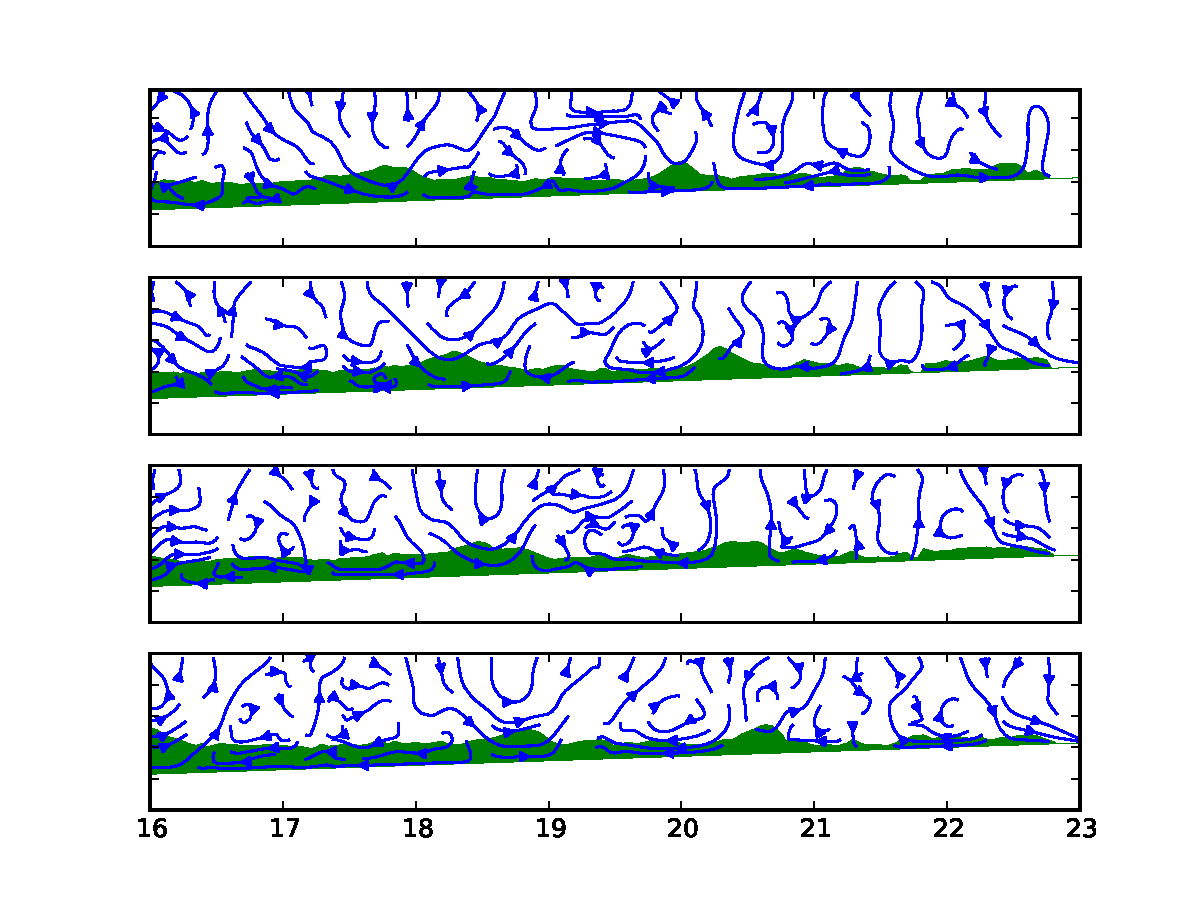
\includegraphics[width=\textwidth]{figures/plunging_breakers.pdf}
\end{frame}

\begin{frame}{Plunging Breakers}
    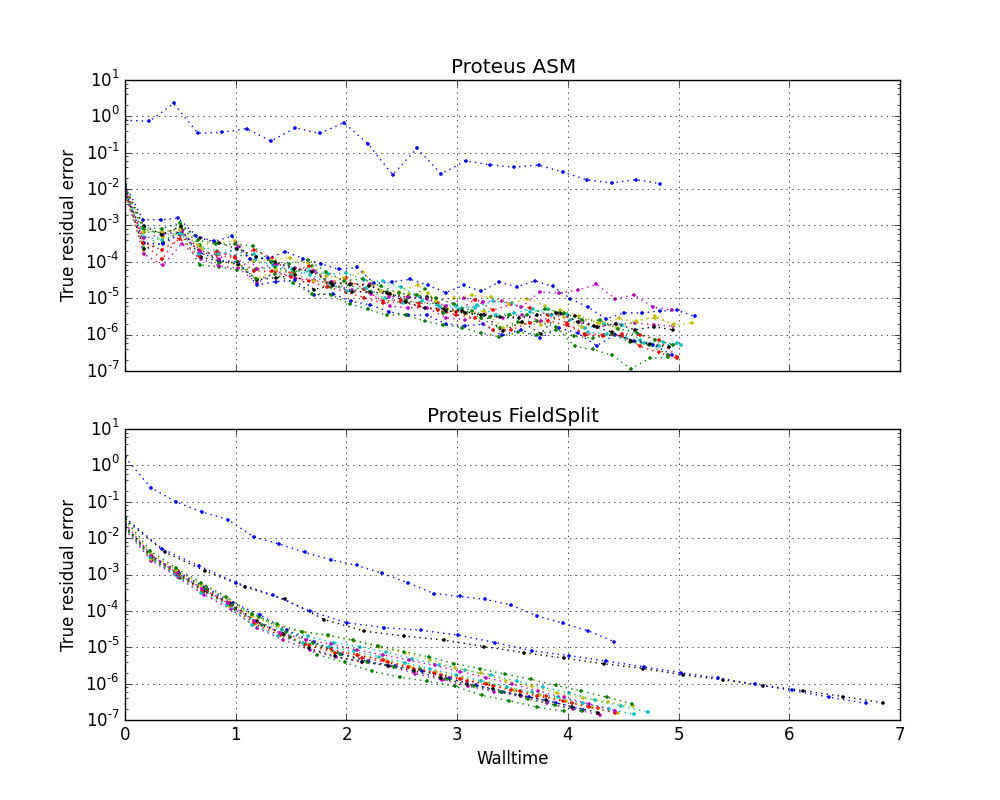
\includegraphics[width=\textwidth]{figures/plunging_comparison.png}
\end{frame}

\begin{frame}{MARIN Benchmark}
    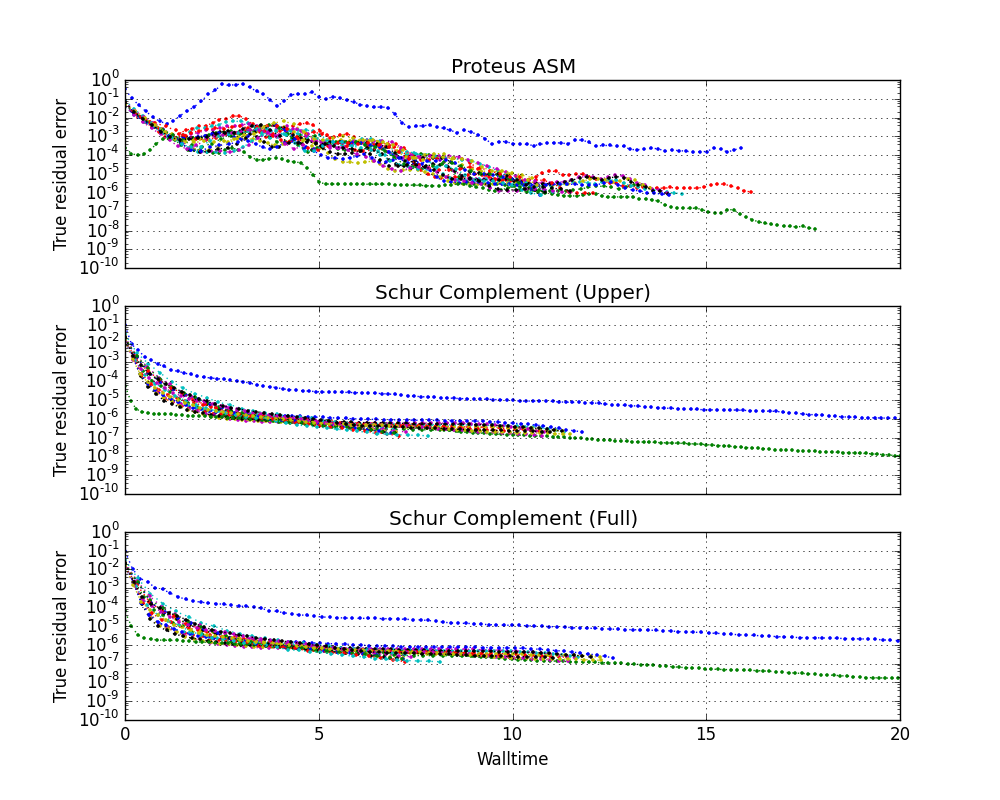
\includegraphics[width=\textwidth]{figures/marin_comparison.png}
\end{frame}

\begin{frame}{Scalability}
    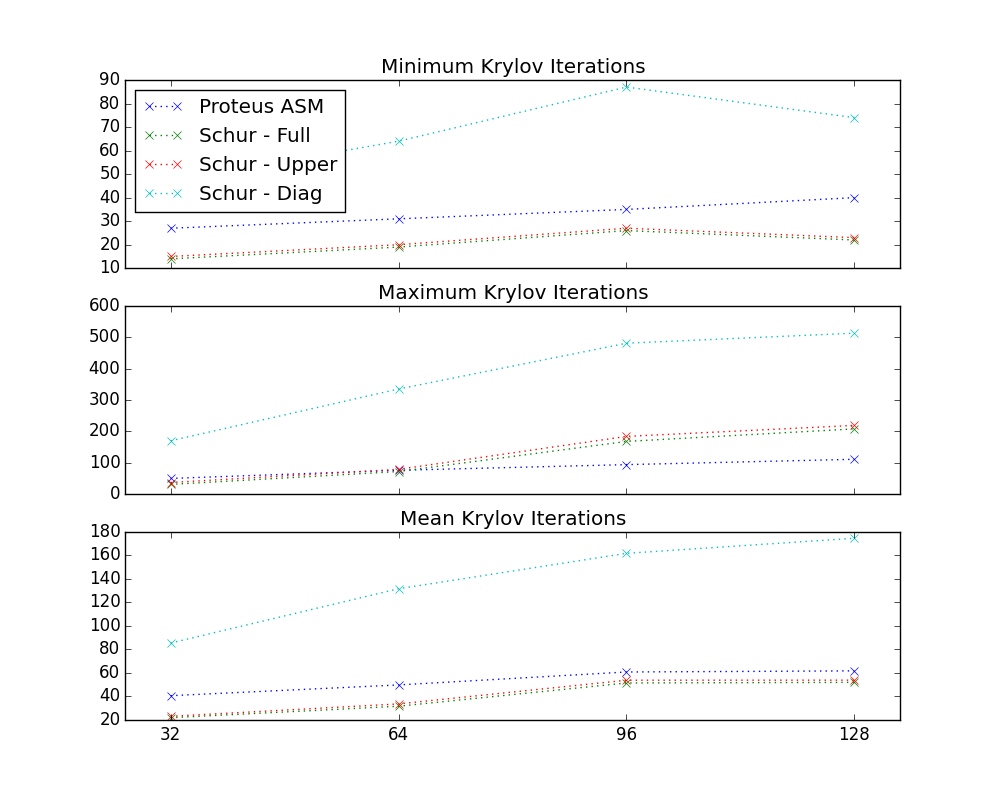
\includegraphics[width=\textwidth]{figures/marin_iterations_scalability.png}
\end{frame}

\begin{frame}{Scalability}
    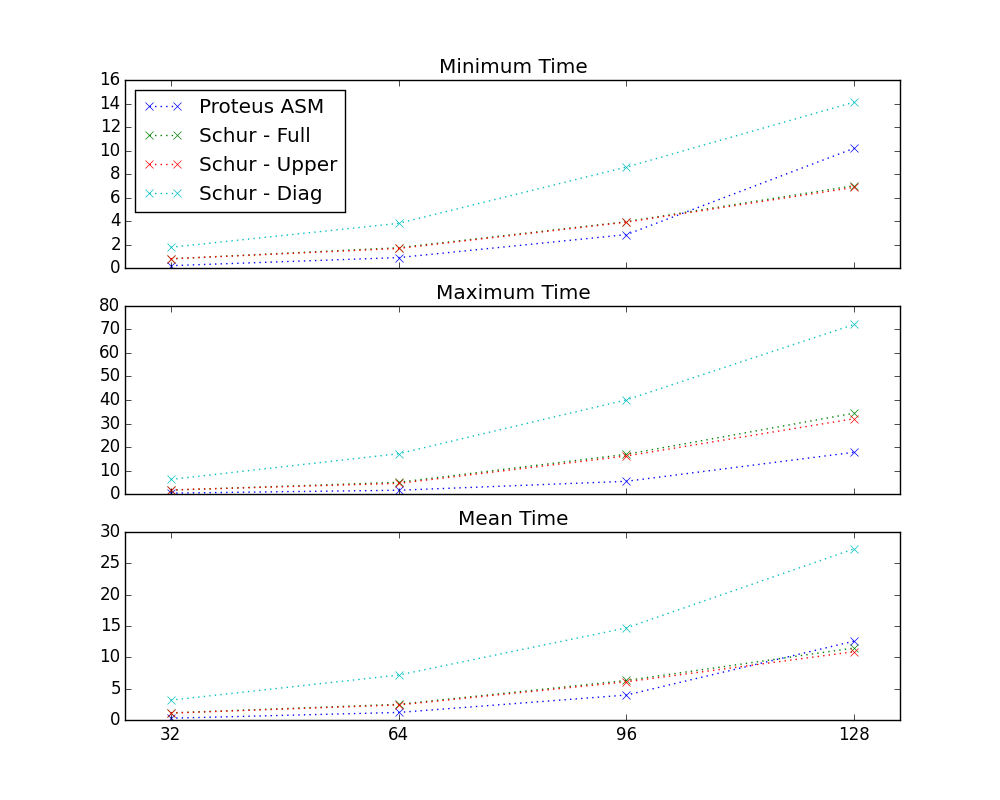
\includegraphics[width=\textwidth]{figures/marin_time_scalability.png}
\end{frame}

\begin{frame}{Conclusion}
  \begin{itemize}
  \item Although the field-split preconditioner requires fewer Krylov
    iterations per solve, the iterations are more expensive
  \item With our current linear system tolerances, the field-split
    preconditioner is only slightly better on the presented problem suite
  \item Looser tolerances could result in performance speedups, but
    this needs to be tested in the application
  \end{itemize}
\end{frame}
\end{document}
